%%%%%%%%%%%%%%%%%%%%%%%%%%%%%%%%%%%%%%%%%
% Beamer Presentation
% LaTeX Template
% Version 1.0 (10/11/12)
%
% This template has been downloaded from:
% http://www.LaTeXTemplates.com
%
% License:
% CC BY-NC-SA 3.0 (http://creativecommons.org/licenses/by-nc-sa/3.0/)
%
%%%%%%%%%%%%%%%%%%%%%%%%%%%%%%%%%%%%%%%%%

%----------------------------------------------------------------------------------------
%	PACKAGES AND THEMES
%----------------------------------------------------------------------------------------

\documentclass{beamer}

\mode<presentation> {

% The Beamer class comes with a number of default slide themes
% which change the colors and layouts of slides. Below this is a list
% of all the themes, uncomment each in turn to see what they look like.

%\usetheme{default}
%\usetheme{AnnArbor}
%\usetheme{Antibes}
%\usetheme{Bergen}
%\usetheme{Berkeley}
%\usetheme{Berlin}
%\usetheme{Boadilla}
%\usetheme{CambridgeUS}
%\usetheme{Copenhagen}
%\usetheme{Darmstadt}
%\usetheme{Dresden}
%\usetheme{Frankfurt}
%\usetheme{Goettingen}
%\usetheme{Hannover}
%\usetheme{Ilmenau}
%\usetheme{JuanLesPins}
%\usetheme{Luebeck}
\usetheme{Madrid}
%\usetheme{Malmoe}
%\usetheme{Marburg}
%\usetheme{Montpellier}
%\usetheme{PaloAlto}
%\usetheme{Pittsburgh}
%\usetheme{Rochester}
%\usetheme{Singapore}
%\usetheme{Szeged}
%\usetheme{Warsaw}

% As well as themes, the Beamer class has a number of color themes
% for any slide theme. Uncomment each of these in turn to see how it
% changes the colors of your current slide theme.

%\usecolortheme{albatross}
%\usecolortheme{beaver}
%\usecolortheme{beetle}
%\usecolortheme{crane}
%\usecolortheme{dolphin}
%\usecolortheme{dove}
%\usecolortheme{fly}
%\usecolortheme{lily}
%\usecolortheme{orchid}
%\usecolortheme{rose}
%\usecolortheme{seagull}
%\usecolortheme{seahorse}
%\usecolortheme{whale}
%\usecolortheme{wolverine}

%\setbeamertemplate{footline} % To remove the footer line in all slides uncomment this line
%\setbeamertemplate{footline}[page number] % To replace the footer line in all slides with a simple slide count uncomment this line

%\setbeamertemplate{navigation symbols}{} % To remove the navigation symbols from the bottom of all slides uncomment this line
}
\usepackage{makecell, cellspace, caption}
\usepackage{longtable}
\usepackage{array}
\usepackage{graphicx} % Allows including images
\usepackage{booktabs} % Allows the use of \toprule, \midrule and \bottomrule in tables

%----------------------------------------------------------------------------------------
%	TITLE PAGE
%----------------------------------------------------------------------------------------
\newcolumntype{L}[1]{>{\raggedright\let\newline\\\arraybackslash\hspace{0pt}}m{#1}}
\newcolumntype{C}[1]{>{\centering\let\newline\\\arraybackslash\hspace{0pt}}m{#1}}
\newcolumntype{R}[1]{>{\raggedleft\let\newline\\\arraybackslash\hspace{0pt}}m{#1}}
\setlength{\parindent}{2em}
\title[Deepfake Detection Using DL]{Deepfake Detection Using Deep Learning} % The short title appears at the bottom of every slide, the full title is only on the title page

\author[ASHOK]{ASHOK V \\
	\medskip
	\text{MDL20CSIP02}
}
\medskip
\institute[MEC] % Your institution as it will appear on the bottom of every slide, may be shorthand to save space
{M.Tech Computer Science and Engineering \\
	with Specialisation in Image Processing \\
	\medskip
	Department of Computer Engineering \\
	\medskip
\text{Government Model Engineering College Thrikkakara}
}
\date{\today} % Date, can be changed to a custom date

\begin{document}

\begin{frame}
\titlepage % Print the title page as the first slide
\end{frame}

\begin{frame}
\frametitle{Overview} % Table of contents slide, comment this block out to remove it
\tableofcontents % Throughout your presentation, if you choose to use \section{} and \subsection{} commands, these will automatically be printed on this slide as an overview of your presentation
\end{frame}

%----------------------------------------------------------------------------------------
%	PRESENTATION SLIDES
%----------------------------------------------------------------------------------------

%------------------------------------------------
 % Sections can be created in order to organize your presentation into discrete blocks, all sections and subsections are automatically printed in the table of contents as an overview of the talk
%------------------------------------------------

 % A subsection can be created just before a set of slides with a common theme to further break down your presentation into chunks
\section{Introduction}
\begin{frame}
\frametitle{Introduction}
\begin{itemize}
	\item Massive expansion of machine learning and	artificial intelligence, any manipulation in images and videos has become possible in recent years.
	\item ML and AI powered deep fake tools have contributed to the creation of fake news and distortion of politicians and celebrities.
	\item Deep learning is an important method in image processing area.
	\item Deep Fakes detection using histogram oriented gradients and support vector machine classifier is exist.
	\item It gave good accuracy on more accurate fakes, but still have problems with low resolution video fakes.
\end{itemize}
\end{frame}

%------------------------------------------------
\section{Literature Survey}
\begin{frame}
\frametitle{Literature Survey}
\begin{center}
\resizebox{\linewidth}{!}{%
	\begin{tabular}{|>{\raggedright\arraybackslash}m{10mm}|m{30mm}|m{60mm}|m{30mm}|m{30mm}|}
		\hline
		\multicolumn{1}{|>{\centering\arraybackslash}m{10mm}|}{\textbf{Sl.No}} &
		\multicolumn{1}{|>{\centering\arraybackslash}m{30mm}|}{\textbf{Paper Details}} &
		\multicolumn{1}{|>{\centering\arraybackslash}m{50mm}|}{\textbf{Methodology}} &
		\multicolumn{1}{|>{\centering\arraybackslash}m{30mm}|}{\textbf{Advantages}} &
		\multicolumn{1}{|>{\centering\arraybackslash}m{30mm}|}{\textbf{Disadvantages}} \\
		\hline
		
		%First Row
		1 &
		Passive Copy- Move Forgery Detection in Videos &
		Copy- Move forgery is a special kind of video forgery technique, in which copy-move of the frame region is performed in intra frame or inter frames. &
		Accuracy is high, Not a complex task &
		Images created using AI can not be detected. Real time detection is not possible \\
		\hline
		
		%Second Row
		2 &
		BusterNet: Detecting Copy-Move Image Forgery with Source/Target Localization &
		BusterNet is a pure, end-to-end trainable, deep neural network solution. It features a two-branch architecture followed by a fusion module. &
		Consist of CNN architecture for each domain (face, iris, and fingerprint) &
		Only works with biometric images \\
		\hline
		
	\end{tabular}
}
\end{center}
\end{frame}

%...............................................

\begin{frame}
	\frametitle{Literature Survey}
	\begin{center}
		\resizebox{\linewidth}{!}{%
			\begin{tabular}{|>{\raggedright\arraybackslash}m{10mm}|m{30mm}|m{60mm}|m{30mm}|m{30mm}|}
				\hline
				\multicolumn{1}{|>{\centering\arraybackslash}m{10mm}|}{\textbf{Sl.No}} &
				\multicolumn{1}{|>{\centering\arraybackslash}m{30mm}|}{\textbf{Paper Details}} &
				\multicolumn{1}{|>{\centering\arraybackslash}m{50mm}|}{\textbf{Methodology}} &
				\multicolumn{1}{|>{\centering\arraybackslash}m{30mm}|}{\textbf{Advantages}} &
				\multicolumn{1}{|>{\centering\arraybackslash}m{30mm}|}{\textbf{Disadvantages}} \\
				\hline
				
				%Third Row
				3 &
				DeepFake Detection on Publicly Available Datasets using Modified AlexNet &
				Used a modified AlexNet constructed of an arrangement of 6 layers. &
				Used 3 publicly available datasets for training. Got a consistent accuracy on these three datasets &
				Accuracy is 87.49\% \\
				\hline
				
				%Fourth Row
				4 &
				Deep Representations for Iris, Face, and Fingerprint Spoofing Detection &
				CNN for detecting the fake iris in biometric images.  &
				First CMFD algorithm with discernibility to localize source/target regions. And it outperforms state-of-the-art copy-move detection algorithms by a large margin on the two publicly available datasets, CASIA and CoMoFoD &
				Real time detection is not possible \\
				\hline
				
			\end{tabular}
		}
	\end{center}
\end{frame}

%------------------------------------------------
\begin{frame}
	\frametitle{Literature Survey}
	\begin{center}
		\resizebox{\linewidth}{!}{%
			\begin{tabular}{|>{\raggedright\arraybackslash}m{10mm}|m{30mm}|m{60mm}|m{30mm}|m{30mm}|}
				\hline
				\multicolumn{1}{|>{\centering\arraybackslash}m{10mm}|}{\textbf{Sl.No}} &
				\multicolumn{1}{|>{\centering\arraybackslash}m{30mm}|}{\textbf{Paper Details}} &
				\multicolumn{1}{|>{\centering\arraybackslash}m{50mm}|}{\textbf{Methodology}} &
				\multicolumn{1}{|>{\centering\arraybackslash}m{30mm}|}{\textbf{Advantages}} &
				\multicolumn{1}{|>{\centering\arraybackslash}m{30mm}|}{\textbf{Disadvantages}} \\
				\hline
				
				%Fifth Row
				5 &
				A Liveness Detection Method for Face Recognition Based on Optical Flow Field &
				The method is based on the assumption that a 3D face generates a special 2-D motion which is higher at central face parts (e.g. nose) compared to the outer face regions (e.g. ears) &
				It recognize spoofing attacks based on the correlation between optical flows in foreground and background regions &
				Works only with videos. And Low accuracy on deepfake dataset \\
				\hline
				
				%Sixth Row
				6 &
				Exposing Deep Fakes Using Inconsistent Head Poses &
				This method is based on the observations that Deep Fakes are created by splicing synthesized face region into the original image, and in doing so, introducing errors that can be revealed when 3D head poses are estimated from the face images. &
				Using features based on this method, an SVM classifier is evaluated using a set of real face images and Deep Fakes. &
				Low accuracy \\
				\hline
				
			\end{tabular}
		}
	\end{center}
\end{frame}
%...............................................
\begin{frame}
	\frametitle{Literature Survey}
	\begin{center}
		\resizebox{\linewidth}{!}{%
			\begin{tabular}{|>{\raggedright\arraybackslash}m{10mm}|m{30mm}|m{60mm}|m{30mm}|m{30mm}|}
				\hline
				\multicolumn{1}{|>{\centering\arraybackslash}m{10mm}|}{\textbf{Sl.No}} &
				\multicolumn{1}{|>{\centering\arraybackslash}m{30mm}|}{\textbf{Paper Details}} &
				\multicolumn{1}{|>{\centering\arraybackslash}m{50mm}|}{\textbf{Methodology}} &
				\multicolumn{1}{|>{\centering\arraybackslash}m{30mm}|}{\textbf{Advantages}} &
				\multicolumn{1}{|>{\centering\arraybackslash}m{30mm}|}{\textbf{Disadvantages}} \\
				\hline
				
				%Seventh Row
				7 &
				Detection of Deep Network Generated Images
				Using Disparities in Color Components &
				This method analyze the disparities in color components between real scene images and deep fake images. Existing deep networks generate images in RGB color space and have no explicit constrains on color correlations; therefore, deep fake images have more obvious differences from real images in other color spaces, such as HSV and YCbCr, especially in the chrominance components. &
				It proposes a  feature set to capture color image statistics for detecting deep fake images. &
				It can not detect deep fakes in videos and need high quality images for detection. \\
				\hline
				
				%Eighth Row
				8 &
				DeepVision: Deepfakes detection using human
				eye blinking pattern &
				It detect Deepfakes generated through the generative adversarial network (GANs) model via an algorithm called DeepVision. It analyze a significant change in the pattern of blinking. &
				Deepfakes can be determined through integrity verification by tracking significant changes in the eye blinking patterns &
				The integrity verification may not be applicable to people with mental illnesses or problems in nerve conduction pathways. \\
				\hline
				
			\end{tabular}
		}
	\end{center}
\end{frame}
%...............................................
\begin{frame}
	\frametitle{Literature Survey}
	\begin{center}
		\resizebox{\linewidth}{!}{%
			\begin{tabular}{|>{\raggedright\arraybackslash}m{10mm}|m{30mm}|m{60mm}|m{30mm}|m{30mm}|}
				\hline
				\multicolumn{1}{|>{\centering\arraybackslash}m{10mm}|}{\textbf{Sl.No}} &
				\multicolumn{1}{|>{\centering\arraybackslash}m{30mm}|}{\textbf{Paper Details}} &
				\multicolumn{1}{|>{\centering\arraybackslash}m{50mm}|}{\textbf{Methodology}} &
				\multicolumn{1}{|>{\centering\arraybackslash}m{30mm}|}{\textbf{Advantages}} &
				\multicolumn{1}{|>{\centering\arraybackslash}m{30mm}|}{\textbf{Disadvantages}} \\
				\hline
				
				%Nineth Row
				9 &
				Exposing Region Splicing Forgeries with Blind Local Noise Estimation &
				Region splicing is a simple and common digital image tampering operation, where a chosen region from one image is composited into another image with the aim to modify the original image’s content &
				It describe a method to expose region splicing by revealing inconsistencies in local noise levels, based on the fact that images of different origins may have different noise characteristics introduced by the sensors or post-processing steps. &
				It can not detect AI generated fake images \\
				\hline
				
				%Tenth Row
				10 &
				Detection of face spoofing using visual dynamics &
				Dynamic mode decomposition,Local binary pattern and support vector machine &
				Fast response and leading to better detection in video attacks &
				Vulnerable to image quality \\
				\hline
				
			\end{tabular}
		}
	\end{center}
\end{frame}
%................................................

\begin{frame}
	\frametitle{Literature Survey}
	\begin{center}
		\resizebox{\linewidth}{!}{%
			\begin{tabular}{|>{\raggedright\arraybackslash}m{10mm}|m{30mm}|m{60mm}|m{30mm}|m{30mm}|}
				\hline
				\multicolumn{1}{|>{\centering\arraybackslash}m{10mm}|}{\textbf{Sl.No}} &
				\multicolumn{1}{|>{\centering\arraybackslash}m{30mm}|}{\textbf{Paper Details}} &
				\multicolumn{1}{|>{\centering\arraybackslash}m{50mm}|}{\textbf{Methodology}} &
				\multicolumn{1}{|>{\centering\arraybackslash}m{30mm}|}{\textbf{Advantages}} &
				\multicolumn{1}{|>{\centering\arraybackslash}m{30mm}|}{\textbf{Disadvantages}} \\
				\hline
				
				%11 Row
				11 &
				Computationally efficient face spoofing detection with motion magnification &
				Eulerian motion maginification, LBP and Histogram of oriented optical flow &
				Efficient for video attacks and it can detect deepfake in real time &
				Less feasible to detect print attacks and 3D spoof models are undetectable \\
				\hline
				
				%12 Row
				12 &
				Face anti-spoofing countermeasure: Efficient 2DMaterials Classification &
				Stokes degree of linear polarization (SDOLP) with polarizer &
				High accuracy in both image and video deep fake. And fast response &
				Very expensive and external hardware is required \\
				\hline
				
				13 &
				Integration of image quality and motion cues for face anti-spoofing: A neural network approach &
				Shearlet based image quality analysis and optical flow map &
				Better performance and fast response &
				Difficult to implement and requires high performance computer to run\\
				\hline
				
			\end{tabular}
		}
	\end{center}
\end{frame}
%................................................

\begin{frame}
	\frametitle{Literature Survey}
	\begin{center}
		\resizebox{\linewidth}{!}{%
			\begin{tabular}{|>{\raggedright\arraybackslash}m{10mm}|m{30mm}|m{60mm}|m{30mm}|m{30mm}|}
				\hline
				\multicolumn{1}{|>{\centering\arraybackslash}m{10mm}|}{\textbf{Sl.No}} &
				\multicolumn{1}{|>{\centering\arraybackslash}m{30mm}|}{\textbf{Paper Details}} &
				\multicolumn{1}{|>{\centering\arraybackslash}m{50mm}|}{\textbf{Methodology}} &
				\multicolumn{1}{|>{\centering\arraybackslash}m{30mm}|}{\textbf{Advantages}} &
				\multicolumn{1}{|>{\centering\arraybackslash}m{30mm}|}{\textbf{Disadvantages}} \\
				\hline
				
				%14 Row
				14 &
				Face2Face Manipulation Detection Based on Histogram of Oriented Gradients &
				This paper uses Histogram Oriented Gradients for feature extraction and Support Vector Machine for classification. &
				Real time detection is possible. It is very simple to implement. &
				The drawback of HOG is that its computation speed is slow while detecting an object and accuracy is not highly reliable compared to the current neural networks \\
				\hline
				
				%15 Row
				15 &
				Xception: Deep Learning with Depthwise Separable Convolution &
				Xception is a deep convolutional neural network architecture that involves Depthwise Separable Convolutions. &
				XCeption is an efficient architecture and give better performance than inception v3,VGG,ResNet &
				It is expensive to train, but are pretty good improvements compared to Inception. Transfer learning brings part of the solution when it comes to adapting such algorithms for a specific task. \\
				\hline
				
			\end{tabular}
		}
	\end{center}
\end{frame}
%................................................
\section{Literature Review}
\begin{frame}
	\frametitle{Literature Review}
	\begin{itemize}
		\item Reviewed some milestone deep learning methods like Histogram Oriented Gradients, InceptionNet, XceptionNet,etc
		\item Using deep learning it is possible to learn robust and high level feature representation of an image
		\item Detecting deep fakes in an image / video is possible with deep learning
		\item Among different deep learning methods, XceptionNet is showing high accuracy and immediate response.
	\end{itemize}
\begin{figure}
	\centering
	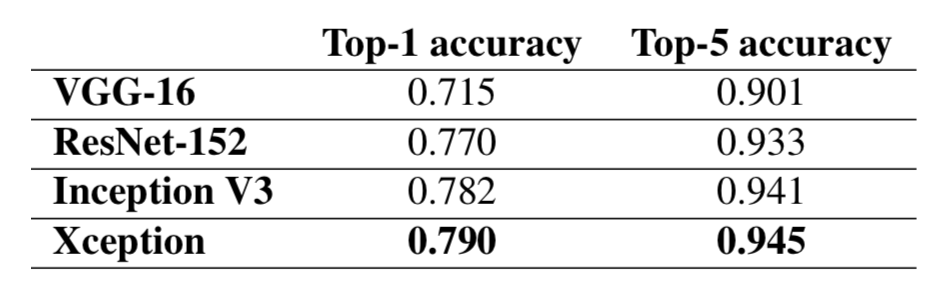
\includegraphics[scale=0.3]{./images/comp.png}
	\caption{Comparison of different architectures}
\end{figure}
\end{frame}
%...............................................
\section{Problem Statement}
\begin{frame}
	\frametitle{Problem Statement}
	A system that automatically and accurately detect deepfakes / faceswaps in images or videos in real time.
\end{frame}

%...............................................

\section{Proposed Solution}
\begin{frame}
	\frametitle{Proposed Solution}
	\begin{figure}
		\centering
		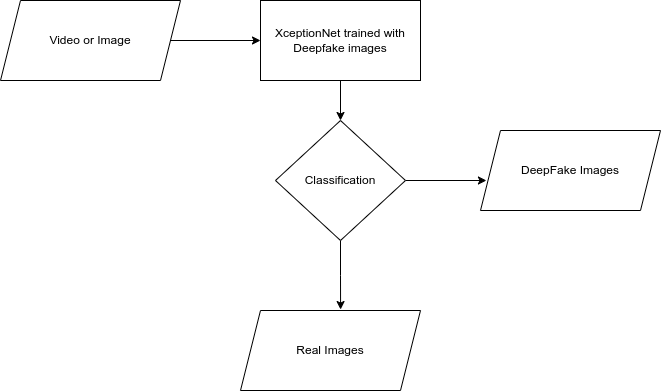
\includegraphics[scale=0.5]{./images/proposed.png}
		\caption{Proposed System}
	\end{figure}
\end{frame}

%...............................................

\section{Work Schedule}
\begin{frame}
	\frametitle{Work Schedule}
	\begin{table}
		\centering
		\def\arraystretch{1.5}%
		\begin{tabular}[!h]{|p{6cm}|p{4cm}|}
			\hline
			Project Design & Feb $4^{th}$ Week \\
			\hline
			Initial Phase & April $4^{th}$ Week \\
			\hline
			Prototype & June $1^{st}$ Week \\
			\hline
			Final Implementation & June $4^{th}$ Week \\
			\hline
		\end{tabular}
	\caption{Tentative Schedule}
	\label{schedule}
	\end{table}
\end{frame}

%...............................................

\section{Hardware and Software Requirements}
\begin{frame}
	\frametitle{Hardware and Software Requirements}
	\begin{table}
		\centering
		\begin{tabular}[!h]{|p{3cm}|p{7cm}|}
			\hline
			\textbf{OS} & Windows 8, 10, Linux \\
			\hline
			\textbf{Software} & Anaconda Python distribution, OpenCV, Numpy, and Deep Learning libraries (Tensorflow, Keras) \\
			\hline
			\textbf{CPU} & Intel core i5 $7^{th}$ generation processor or higher or an AMD equivalent processor \\
			\hline
			\textbf{RAM} & 8GB \\
			\hline
			\textbf{GPU} & 4GB \\
			\hline
			\textbf{Disk Storage} & 50 GB of free disk space \\
			\hline
		\end{tabular}
		\caption{Hardware and Software Requirements}
		\label{requirements}
	\end{table}
\end{frame}

%-------------------------------------------------------------------------



%------------------------------------------------



%------------------------------------------------



%------------------------------------------------



%------------------------------------------------


%------------------------------------------------
\section{References}
\begin{frame}
\frametitle{References}
\footnotesize{
\begin{thebibliography}{99} % Beamer does not support BibTeX so references must be inserted manually as below
\bibitem[1]{p1} Pandey, Ramesh Chand, Sanjay Kumar Singh, and K. K. Shukla (2014)
\newblock Passive copy-move forgery detection in videos
\newblock \emph{International conference on computer and communication technology (ICCCT). IEEE}.

\bibitem[2]{p1} Wu, Yue, Wael Abd-Almageed, and Prem Natarajan (2018)
\newblock Busternet: Detecting copy-move image forgery with source/target localization
\newblock \emph{Proceedings of the European Conference on Computer Vision (ECCV)}.

\bibitem[3]{p1}Xie, Daniel (2020)
\newblock DeepFake Detection on Publicly Available Datasets using Modified AlexNet
\newblock \emph{2020 IEEE Symposium Series on Computational Intelligence (SSCI)}.

\bibitem[4]{p1}Menotti, David (2015)
\newblock Deep representations for iris, face, and fingerprint spoofing detection
\newblock \emph{IEEE Transactions on Information Forensics and Security 10.4}.
\end{thebibliography}
}
\end{frame}

%------------------------------------------------

\begin{frame}
	\frametitle{References}
	\footnotesize{
		\begin{thebibliography}{99} % Beamer does not support BibTeX so references must be inserted manually as below
			\bibitem[5]{p1} Bao, Wei (2009)
			\newblock A liveness detection method for face recognition based on optical flow field
			\newblock \emph{2009 International Conference on Image Analysis and Signal Processing. IEEE}.
			
			\bibitem[6]{p1} Yang, Xin, Yuezun Li, and Siwei Lyu (2019)
			\newblock Exposing deep fakes using inconsistent head poses
			\newblock \emph{ICASSP 2019-2019 IEEE International Conference on Acoustics, Speech and Signal Processing (ICASSP). IEEE}.
			
			\bibitem[7]{p1}Li, H (2018)
			\newblock Detection of deep network generated images using disparities in color components. arXiv 2018
			\newblock \emph{arXiv preprint arXiv:1808.07276}.
			
			\bibitem[8]{p1}Jung, Tackhyun, Sangwon Kim, and Keecheon Kim (2020)
			\newblock DeepVision: deepfakes detection using human eye blinking pattern
			\newblock \emph{IEEE Access 8 (2020): 83144-83154}.
		\end{thebibliography}
	}
\end{frame}

%................................................
\begin{frame}
	\frametitle{References}
	\footnotesize{
		\begin{thebibliography}{99} % Beamer does not support BibTeX so references must be inserted manually as below
			\bibitem[9]{p1} Lyu, Siwei, Xunyu Pan, and Xing Zhang (2014)
			\newblock Exposing region splicing forgeries with blind local noise estimation
			\newblock \emph{International journal of computer vision 110.2 (2014): 202-221}.
			
			\bibitem[10]{p1} YFerrara, Pasquale, et al (2012)
			\newblock Image forgery localization via fine-grained analysis of CFA artifacts
			\newblock \emph{IEEE Transactions on Information Forensics and Security 7.5 (2012): 1566-1577}.
			
			\bibitem[11]{p1}Megahed, Amr, and Qi Han (2020)
			\newblock Face2Face Manipulation Detection Based on Histogram of Oriented Gradients.
			\newblock \emph{2020 IEEE 19th International Conference on Trust, Security and Privacy in Computing and Communications (TrustCom)}.
			
			\bibitem[12]{p1}Jung, Tackhyun, Sangwon Kim, and Keecheon Kim (2020)
			\newblock DeepVision: deepfakes detection using human eye blinking pattern
			\newblock \emph{IEEE Access 8 (2020): 83144-83154}.
		\end{thebibliography}
	}
\end{frame}
%................................................
\begin{frame}
\Huge{\centerline{Thank You !}}
\end{frame}

%----------------------------------------------------------------------------------------

\end{document} 